%coding:utf-8

%----------------------------------------
%FOSAPHY, a LaTeX-Code for a summary of optics
%Copyright (C) 2014, Mario Felder, Michael Fallegger

%This program is free software; you can redistribute it and/or
%modify it under the terms of the GNU General Public License
%as published by the Free Software Foundation; either version 2
%of the License, or (at your option) any later version.

%This program is distributed in the hope that it will be useful,
%but WITHOUT ANY WARRANTY; without even the implied warranty of
%MERCHANTABILITY or FITNESS FOR A PARTICULAR PURPOSE.  See the
%GNU General Public License for more details.
%----------------------------------------

\chapter{Strahlen Optik}

\section{Einleitung}
\begin{itemize}
	\item Einfallswinkel = Ausfallswinkel 
	\item Licht breitet sich von einem Punkt A zu einem Punkt B so aus, dass die Laufzeit minimal wird. \\
\end{itemize}
\
\section{Konstanten}
\[
\boxed{\begin{aligned}	
		&\text{Lichtgeschwindigkeit} \\
		&c = 299'792'458\text{ m/s}\\
	\end{aligned}}	\]
\\
\\
\section{Brechung und Brechungsindex n}
Brechungsindex: 
\[
	n= \frac{c}{c_{mat}}
\]
Brechungsgesetz von Snellius: 
\[
	n_A \cdot \sin \theta_A = n_B\cdot \sin \theta_B
\]

\begin{footnotesize}
	Der \textbf{Winkel} bezüglich der Grenzfläche-Lots.
\end{footnotesize}
\\
\\
\section{Strahlenverschiebung}
\[
	\Delta x = d \cdot \frac{ \sin (\theta_a -\theta_b ^`)}{\cos \theta_b ^`}
\]
\begin{center}
	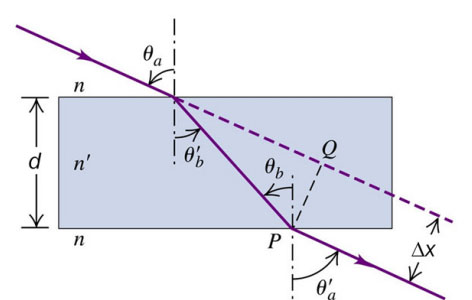
\includegraphics[scale = 0.3]{../fig/strahlenverschiebung.jpg}
\end{center}
\

\section{Totalreflexion}
Totalreflexion tritt auf, wenn der Grenzwinkel $\theta_krit$ überschritten wird.
\[
	\sin \theta_{krit} = \frac{n_B}{n_A}
\]
Totalreflexion Prisma:
\[
	\sin\frac{\alpha+\delta}{2} = n\cdot \sin \frac{\alpha}{2}
\]
\begin{center}
	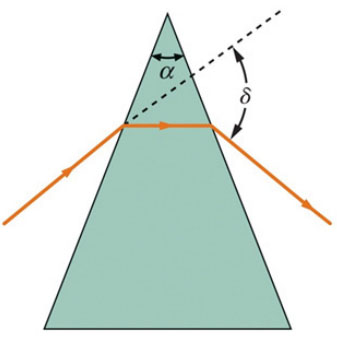
\includegraphics[scale = 0.2]{../fig/tr_prisma.jpg}
\end{center}
\
\section{Linsen}
\textbf{Sammellinsen, Konvexlinsen:} 
Dieser Linsentyp hat eine positive d.h. reelle Brennweite
\\
\textbf{Zerstreulinsen, Konkavlinsen:} 
Dieser Linsentyp hat eine negative, d.h. virtuelle Brennweite f

\subsection{Strahlkonstruktion bei dünnen Linsen}
Linsengleichung:
\[
	\frac{1}{f} = \frac{1}{g} + \frac{1}{b} \\
	\Rightarrow \\
	b=\frac{f \cdot g}{g -f} \\ \\
\]
\[
	\frac{B}{G} =\frac{b}{g}
\]
\begin{center}
	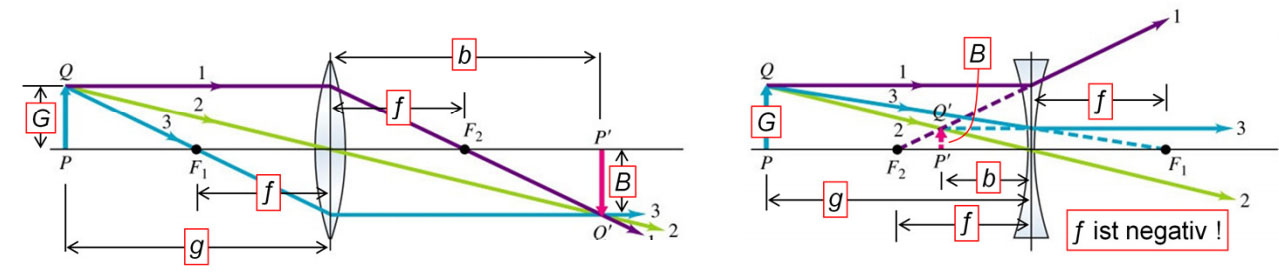
\includegraphics[scale = 0.25]{../fig/strahlkonstruktion.jpg}
\end{center}

\subsection{Vergrösserung}
Vergrösserung:
\[
	M=\frac{\theta^`}{\theta}= \frac{g_{NP}}{f} \approx \frac{25cm}{f}
\]
\begin{center}
	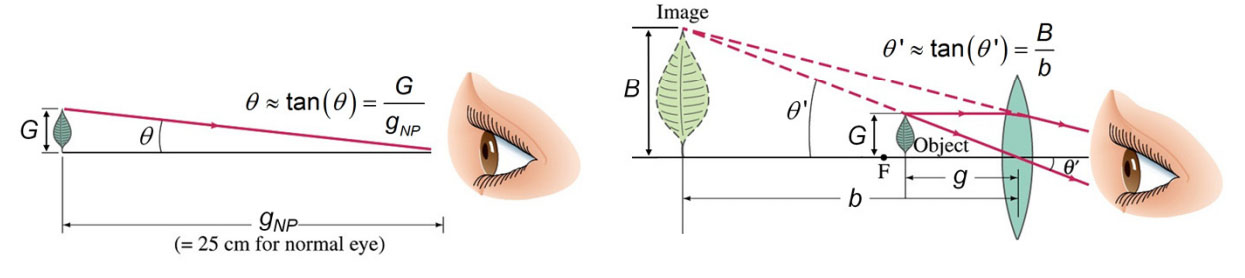
\includegraphics[scale = 0.25]{../fig/vergroesserung.jpg}
\end{center}

\subsection{Optische Instrumente: Mikroskop}
Vergrösserung eines Mikroskops:
\[
	M=m_1 \cdot m_2 = \frac{L\cdot g_{NP}}{f_0 \cdot f_e}
\]
\begin{center}
	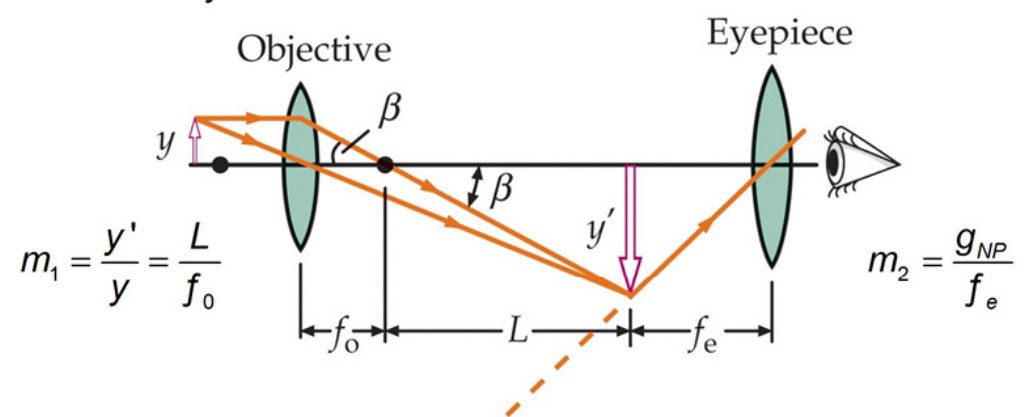
\includegraphics[scale = 0.2]{../fig/mikroskop.jpg}
\end{center}


